%%% PREAMBLE
\documentclass[12pt, a4paper]{article}
%% Packages
% Layout 
\usepackage{parskip} % Changes parskip from being indent-based to adding vertical space
\usepackage[margin=2.5cm]{geometry} % Adjust margins to comply with 2,5cm standard
\usepackage{float}
\usepackage{pdflscape}
\usepackage{listings}

% 
\usepackage[utf8]{inputenc}
\usepackage[T1]{fontenc}

% Font management (for math and normal text)
\usepackage{lmodern} % Changes font to Latin Modern
\usepackage{amssymb, amsmath, amsthm} % Adds math functionality, fonts and environments

% Bibliography and comment management
\usepackage[backend=biber,style=nature]{biblatex} % Bibliography management
\addbibresource{bibliography.bib} % Sets the bibliography-file
\usepackage{csquotes} % Adds babel-biliography compatability 
\usepackage{comment} % Comments package for citation-purposes

% Appendix, attachments management
\usepackage[toc,page]{appendix} %
\renewcommand{\appendixtocname}{Appendiks}
\renewcommand{\appendixpagename}{Appendiks}
\usepackage{pdfpages} % Including PDF-pages
    \usepackage{eso-pic}
    \usepackage{atbegshi}
    \usepackage{ifthen}
    \usepackage{calc}
    
    % miscellaneous
    \usepackage[danish]{translator}
    \usepackage[danish]{babel} % Multi-lingual support - danish
    \usepackage{lipsum} % Adds lipsum functionality
    \usepackage{graphicx} %Titlepage - graphic support
    \usepackage[colorlinks = true,linkcolor = blue,urlcolor  = blue,citecolor = blue,anchorcolor = blue]{hyperref} %Titlepage - customizes hyperlinks
    \usepackage{pgfgantt} % Gantt-Diagram management
    \ganttset{calendar week text={Uge~\currentweek}}
    \usepackage{tikz}
    \usepackage{mdframed}

\usepackage{dirtree}    

%%% Document management
\begin{document}
%% Front matter
    \pagenumbering{roman}
    \begin{titlepage}
    \centering

    \vspace*{1cm}

    % Title and subtitle are enclosed between two rules.
    \rule{\textwidth}{1pt}

    % Title
    \vspace{.7\baselineskip}
    {\huge \textbf{Projekt - studiemiljø}}

    % Subtitle
    \vspace*{.5cm}
    {\LARGE Forårssemester 2024}
    
    \rule{\textwidth}{1pt}

    \vspace{1cm}

    % Set this size for the remaining titlepage.
    \large

    % Authors side by side, using two minipages as a trick.

    \begin{table}[h]
        \begin{tabular}{lr}
            \begin{minipage}{.5\textwidth}
                \centering
                Jeppe Bøgeskov Bech\\
                {\normalsize \url{jepp9920@zbc.dk}}
            \end{minipage}%
        &      
            \begin{minipage}{.5\textwidth}
                \centering
                Alexander Schade Knudsen \\
                {\normalsize \url{alex245h@zbc.dk}}
            \end{minipage}
            \vspace{1cm}
         \\ 
            \begin{minipage}{.5\textwidth}
                \centering
                Andreas Jensen \\
                {\normalsize \url{andr328q@zbc.dk }}
            \end{minipage} 
         & 
            \begin{minipage}{.5\textwidth}
                \centering
                David Rasmussen\\
                {\normalsize \url{davi5621@zbc.dk}}
            \end{minipage}
        \end{tabular}
    \end{table}





    

    % More authors can be inserted here with additional minipages.

    \vspace{1cm}

    % Report logo.
    
\includegraphics[width=.7\textwidth]{./assets/zbc_logo_black.jpg}

    \vfill

    % University and date information at the bottom of the titlepage.
    1. x \\
    ZBC Handels- og Teknisk gymnasium Slagelse \\
    Akademisk år 2023-2024 \\
    \today
\end{titlepage}
    \newpage
    \section{Indledning}
    Denne rapport henvender sig til de relevante faglærer og dokumenterer teknologiprojektet i forårssemesteret. 

    Forneden gennemgås strukturen samt nogle af designvalgene bag opsætningen af rapporten.

    Dokumentet er skrevet med fonten \textit{Latin Modern}, grundet dens kompatibilitet med diverse matematik, sprog og symboler, med matematik i skriftstørrelsen 12pt. Præliminærsiderne er pagineret med romertal, brødteksten med arabiske tal og appendikssiderne med dets bogstav samt de arabiske tal.

    Dokumentet er typesat via \LaTeX, et markup-sprog, da det tillader for utroligt smukke dokumenter, nem numerering samt administration af figurer, tabeller, bibliografier og appendikser. \TeX-kodefilerne kan tilgås via GitHub, ligedan med kodedelen af projektet: \url{https://github.com/ZBC-Slagelse-HTX-X/Teknologi-project}.

    Dokumentet er opdelt i tre hovedkapitler:
    \begin{itemize}
        \item Opgavevalg (\ref{sec:opgavevalg}), hvori opgavekrav og oplæg slås fast--derved fundamentet for projektet.
        \item Projektstyring (\ref{sec:projektstyring}), hvori ansvarsområdedelegation  og praktisk information som tidsplanen kan findes.
        \item Projektudvikling (\ref{sec:projektudvikling}), hvori den reelle projektudvikling dokumenteres.
    \end{itemize}
    \newpage
    \tableofcontents
    \newpage
%% Main body
    \pagenumbering{arabic}
    %%% Introduction to project
\section{Opgavevalg \label{sec:opgavevalg}}
    \subsection{Formål og opgavekrav}
        Teknologiprojektet beskrevet heri omhandler HTX' studiemiljø, hvortil der er tre oplæg.  
    \subsection{Oplæg}
         \newpage
    \section{Projektstyring}
    \begin{landscape}
        \subsection{Tidsplan}
            \begin{figure}[H]
    \resizebox{\columnwidth}{!}{%
    \begin{ganttchart}{1}{60}
        \gantttitle{2024}{60} \\
        \gantttitle{Marts}{30} \gantttitle{April}{30} \\
        \gantttitlelist{1,...,30}{1} \gantttitlelist{1,...,30}{1}\\
        \ganttgroup{Forberedelse}{1}{6} \\
        \ganttbar{Projektbeskrivelse}{1}{6} \\
        \ganttlinkedbar{Task 2}{3}{7} \ganttnewline
        % \ganttmilestone{Milestone}{7} \ganttnewline
        % \ganttbar{Final Task}{8}{12}
        % \ganttlink{elem2}{elem3}
        % \ganttlink{elem3}{elem4}
    \end{ganttchart}}
    \caption{Viser Gantt-Diagram over vores foreløbige tidsplan}
\end{figure}
    \end{landscape}
    \subsection{Rollefordeling}
        \begin{tabular}{r|r|r}
            Navn & Ansvarsområde &  \\ \hline
            Jeppe &  Kodning \\ \hline
            Alexander  & $\mathrm{\latex}$ \& opstilling \\ \hline
            Andreas & Hardware   \\ \hline
            David &  Logging \\ \hline
        \end{tabular} \newpage
    \section{Projektudvikling \label{sec:Projektudvikling}}
    \subsection{Lectio renovering}
        \subsubsection{Overordnet}
                        
    \subsection{Smartdøre}
        \subsubsection{Software}
        \subsection{Hardware}
    \subsection{Booking system} \newpage

    \section{Produktprincip}
    \subsection{Målgruppe}
    Efter som det nuværende Lectio bliver anvendt af en stor del af landets gymnasier, er vores målgruppe derved alle landets gymnasier--nemlig også potentielle kunder (gymnasier) der
    muligvis ville være interesseret i at anvende vores Lectio applikation. 
    
    Målgruppen for RFID-Systemet er ligeledes gymnasielle udannelser.

    \subsection{Kravspecifikation}
    \subsubsection{Krav til Lectio rework}
    Kravene for vores applikation er følgende: 
    \begin{itemize}
        \item Applikationen skal have alle de samme core-features som det originale Lectio
        \item Applikationen skal være let overskuelig og nemt orienterbart for brugerne
        \begin{itemize}
            \item Applikationen skal således være simplere end sin forløber
        \end{itemize}
        \item Applikationen skal indeholde et Lokale-Booking-System/Fraværsregistreringssystem/Dørsystem 
        \begin{itemize}
            \item Applikationen skal have forbedret fraværsregistrering
            \item Applikationen skal give alle eleverne et digitalt persona i sammenspil med fraværsregistreringssystemet. 
            \item Et komplet dørsystem som låses/låses op med RFID kort (på sigt ens mobiltelefon). 
        \end{itemize}
    \end{itemize}
    
    \subsubsection{Krav til RFID-System}
    Kravene til RFID-Systemet er følgende:
    \begin{itemize}
        \item Systemet skal gøre det nemt for elever at booke lokaler de skal bruge til undervisningsformål.
        \item Systemet skal hjælpe med at forbedre fraværsregistrering og spare tid i timerne. 
        \item Systemet skal gøre det muligt i tilfælde af brand på skolens premis at sikre flugtveje. 
        \item Systemet skal gøre det muligt i tilfælde af brand at have styr på alle elever.
        \item Systemet skal være nemt at bruge og ikke skabe forvirring.
    \end{itemize}
    

    \subsection{Kort om konkurrenter}
        Lectio har ingen umiddelbare konkurrenter, vi kender, udover Aula, men det henvender sig til 
        folkeskoler og har ikke envidere fildelingsinfrastruktur. Vi tror også, at problemet med Lectio 
        stammer fra det faktum, at Lectio har et de-facto monopol på IT-løsninger målrettet gymnasier.
        \newline
        \newline
        Der findes allerade utallige virksomheder som levere døre med RFID-Låse, dog kan disse ikke implementeres med
        en online applikation som vores.

    \subsection{Løsningsforslag}
        \subsubsection{Lectio rework}
        For at løse problemet med det forældede Lectio har vi besluttet at lave et komplet rework (dvs. genopbyggelse af softwaren, men med samme kernefunktionalitet) af Lectio applikationen.

        Vi har udarbejdet skitser for at kvalificerer vores produktudformning. Sktitserne viser de vigtigste sider af vores Lectio rework.
        \begin{figure}[H]
            \centering
            \resizebox{!}{12cm}{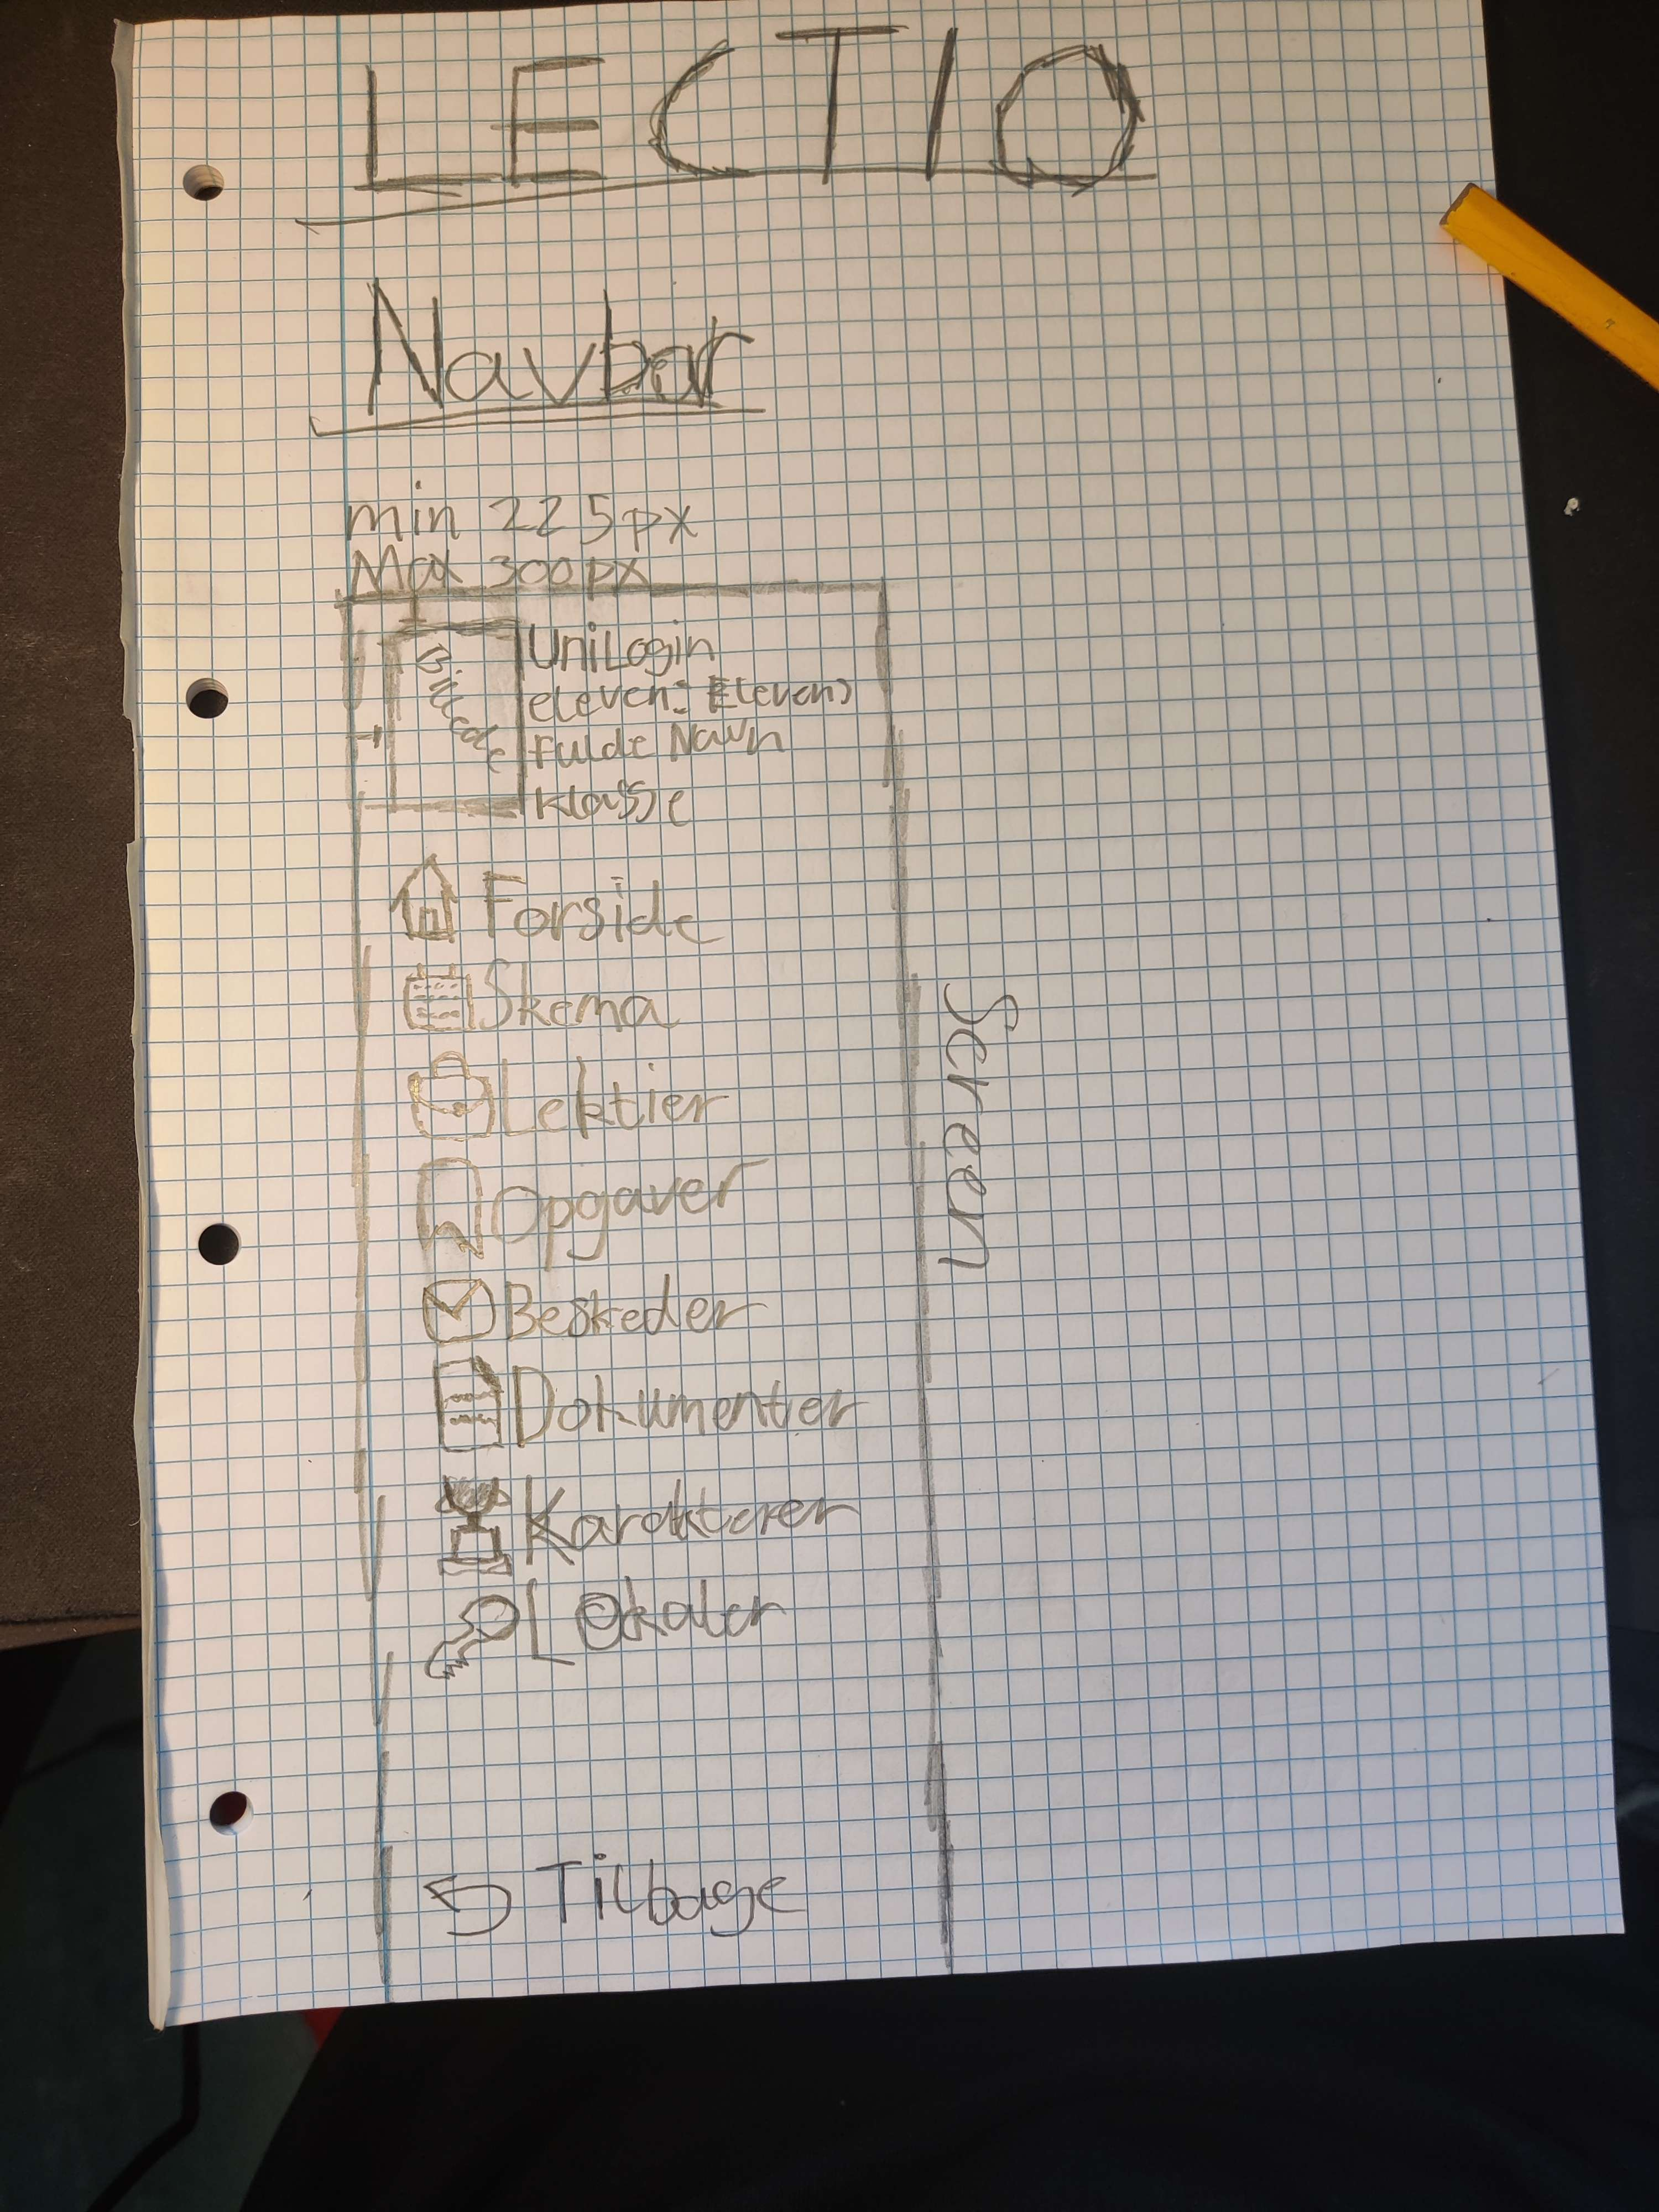
\includegraphics[]{assets/lectio_navbar_skitse.jpg}}
            \caption{Viser Lectioreworkets navigationsbarkomponent - bjælken, brugeren intergerer med}
        \end{figure}

        \begin{figure}[H]
            \centering
            \resizebox{!}{10cm}{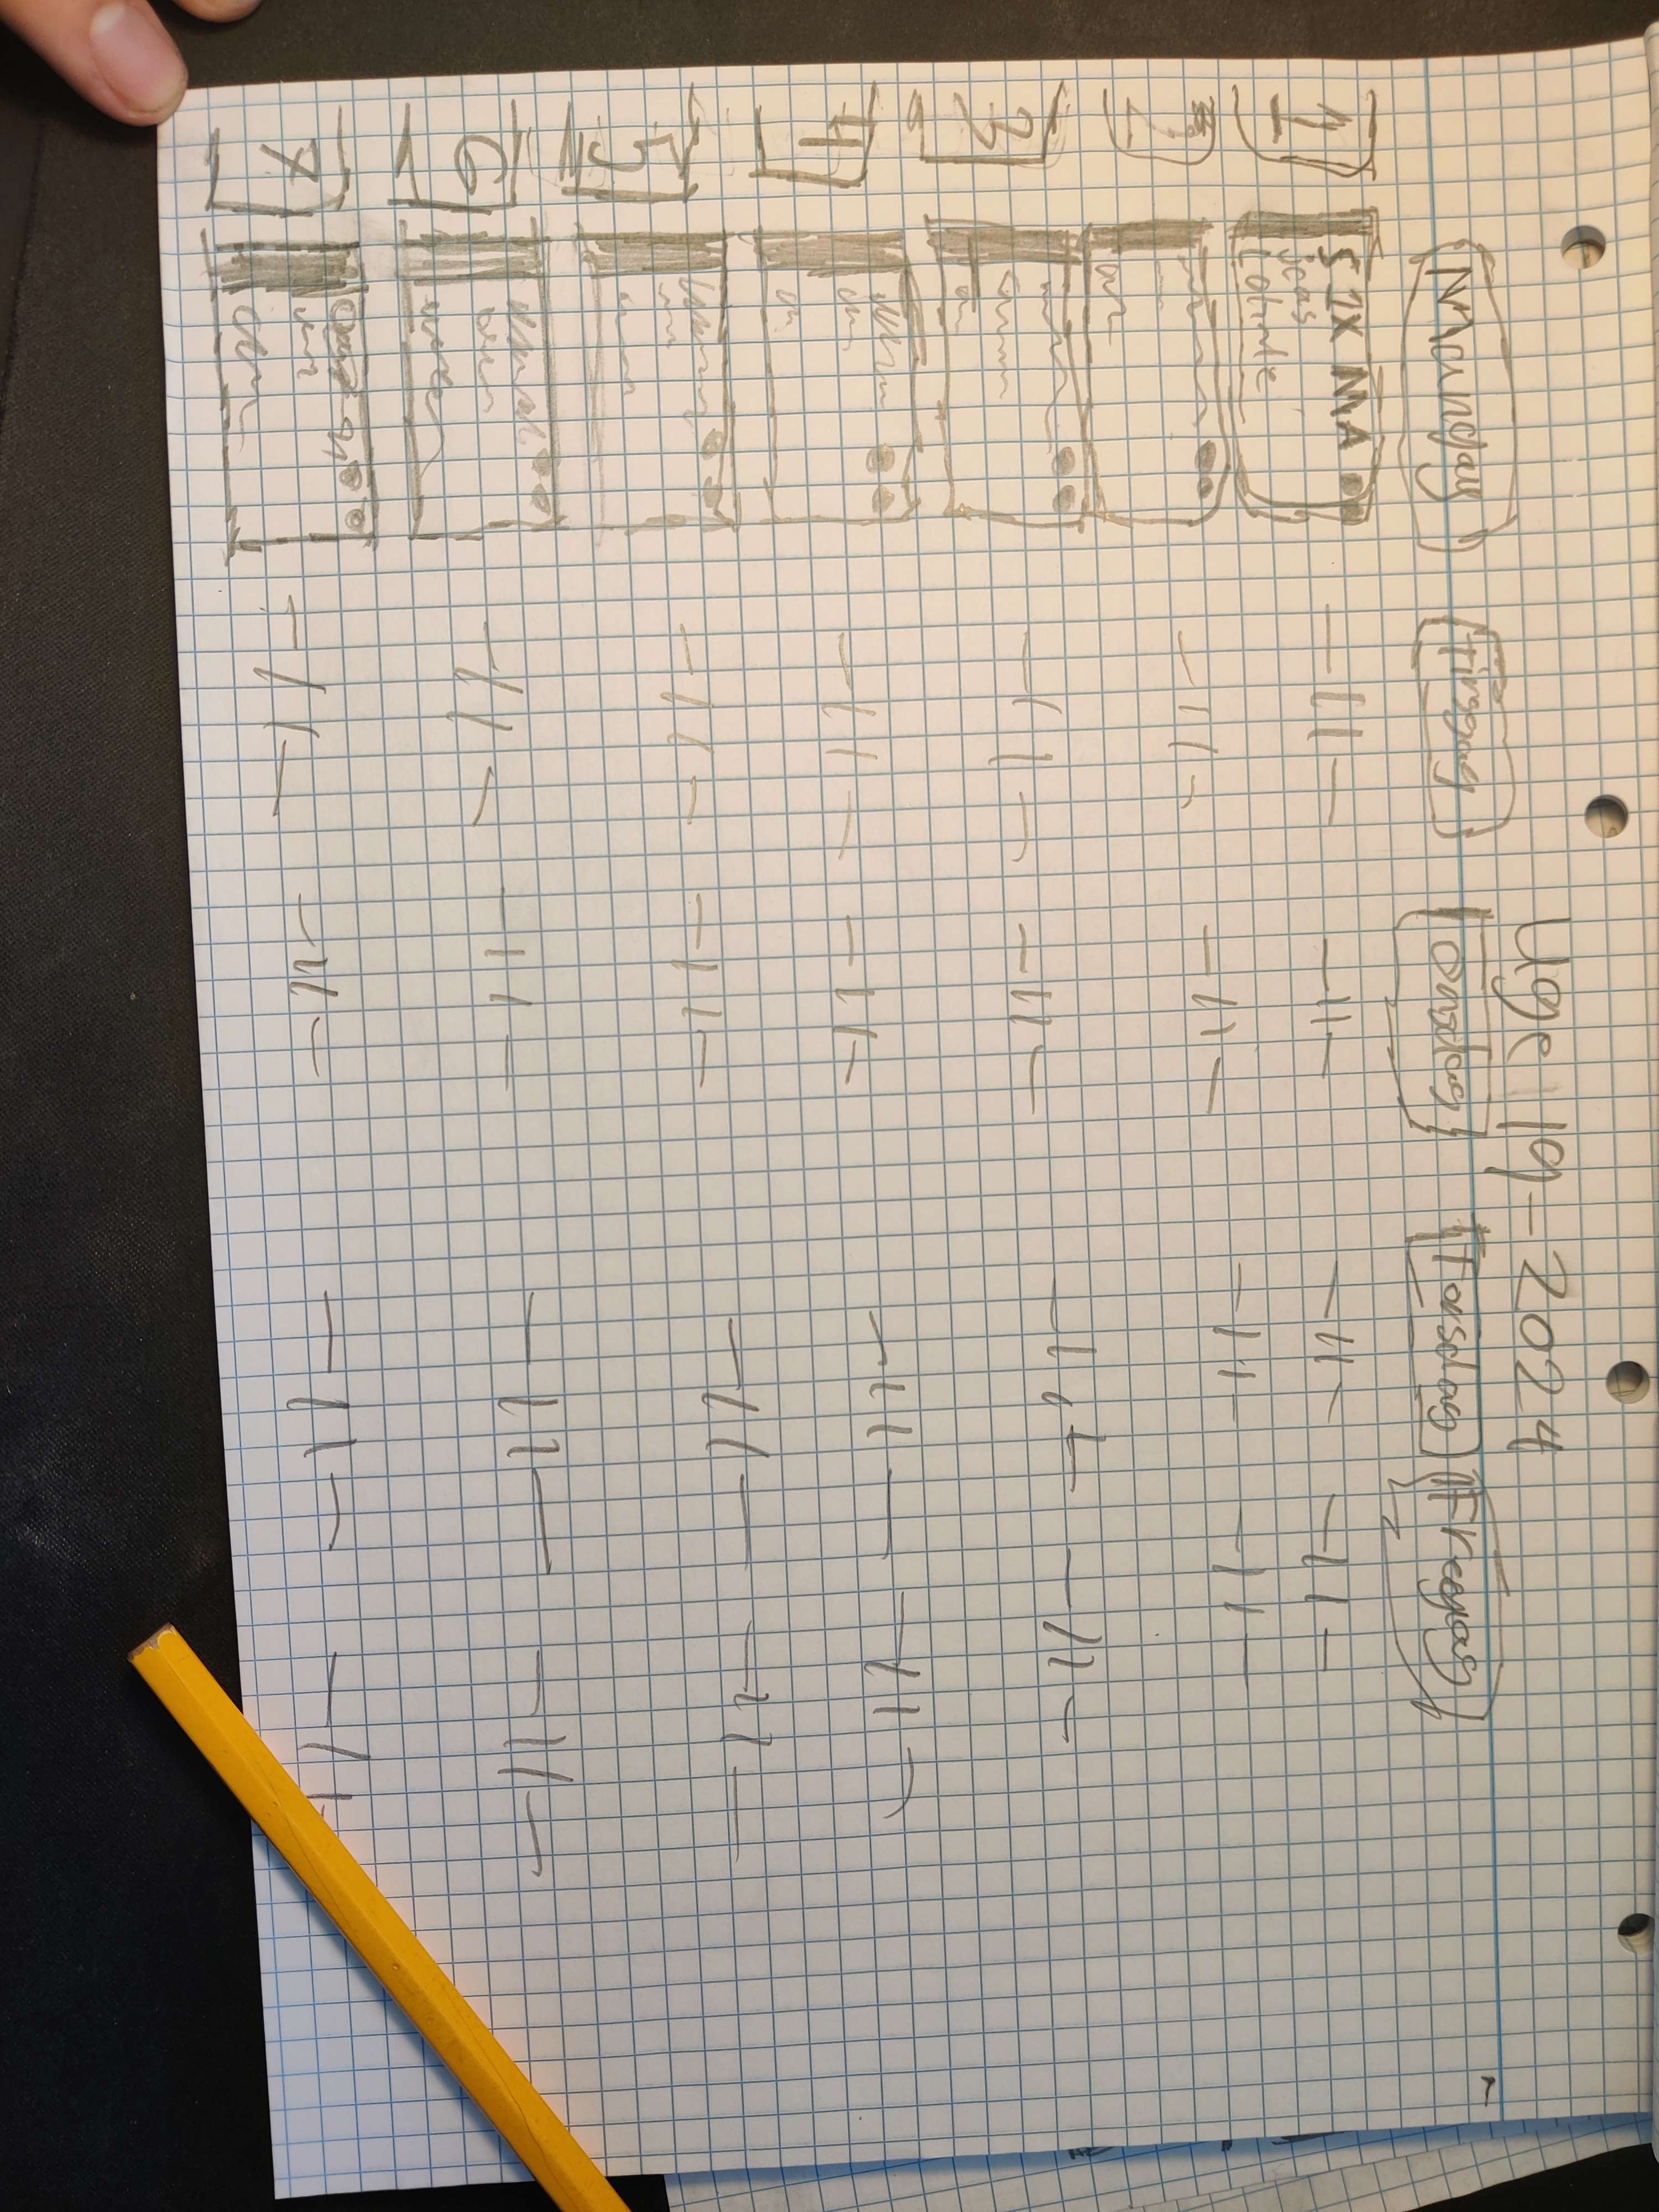
\includegraphics[angle =90]{assets/lectio_skema_skite.jpg}}
            \caption{Viser Lectioreworkets skema side}
        \end{figure}

        De resterende skitser, vi har udarbejdet, fremgår af appendikssektionen \ref{appendix:arbejdsskitser}.

        \subsubsection{RFID-Løsning}
        For at tage hånd om problemet med spildtid i form af fraværstagning, fejlagtig fraværstagning m.v. har vi valgt at lave et dør/fraværssystem, som når man om morgnen møder ind, scanner man sig ind med sit ID-kort eller sit
        digitale ID-kort med sin mobiltelefon på fraværsregistreringssystemet som er i klassen.  
        Lokale-Booking-Systemet fungerer (i ideen--se evalueringen \ref{sec:konklusion}) i sammenspil med den nye Lectio applikation, så kan igennem applikationen booke et lokale også med sit ID-kort
        låse lokalet op i det tidsrum man har booket det pågældene lokale. Web løsningen ses skitseret forneden:

        \begin{figure}[H]
            \centering
            \resizebox{!}{10cm}{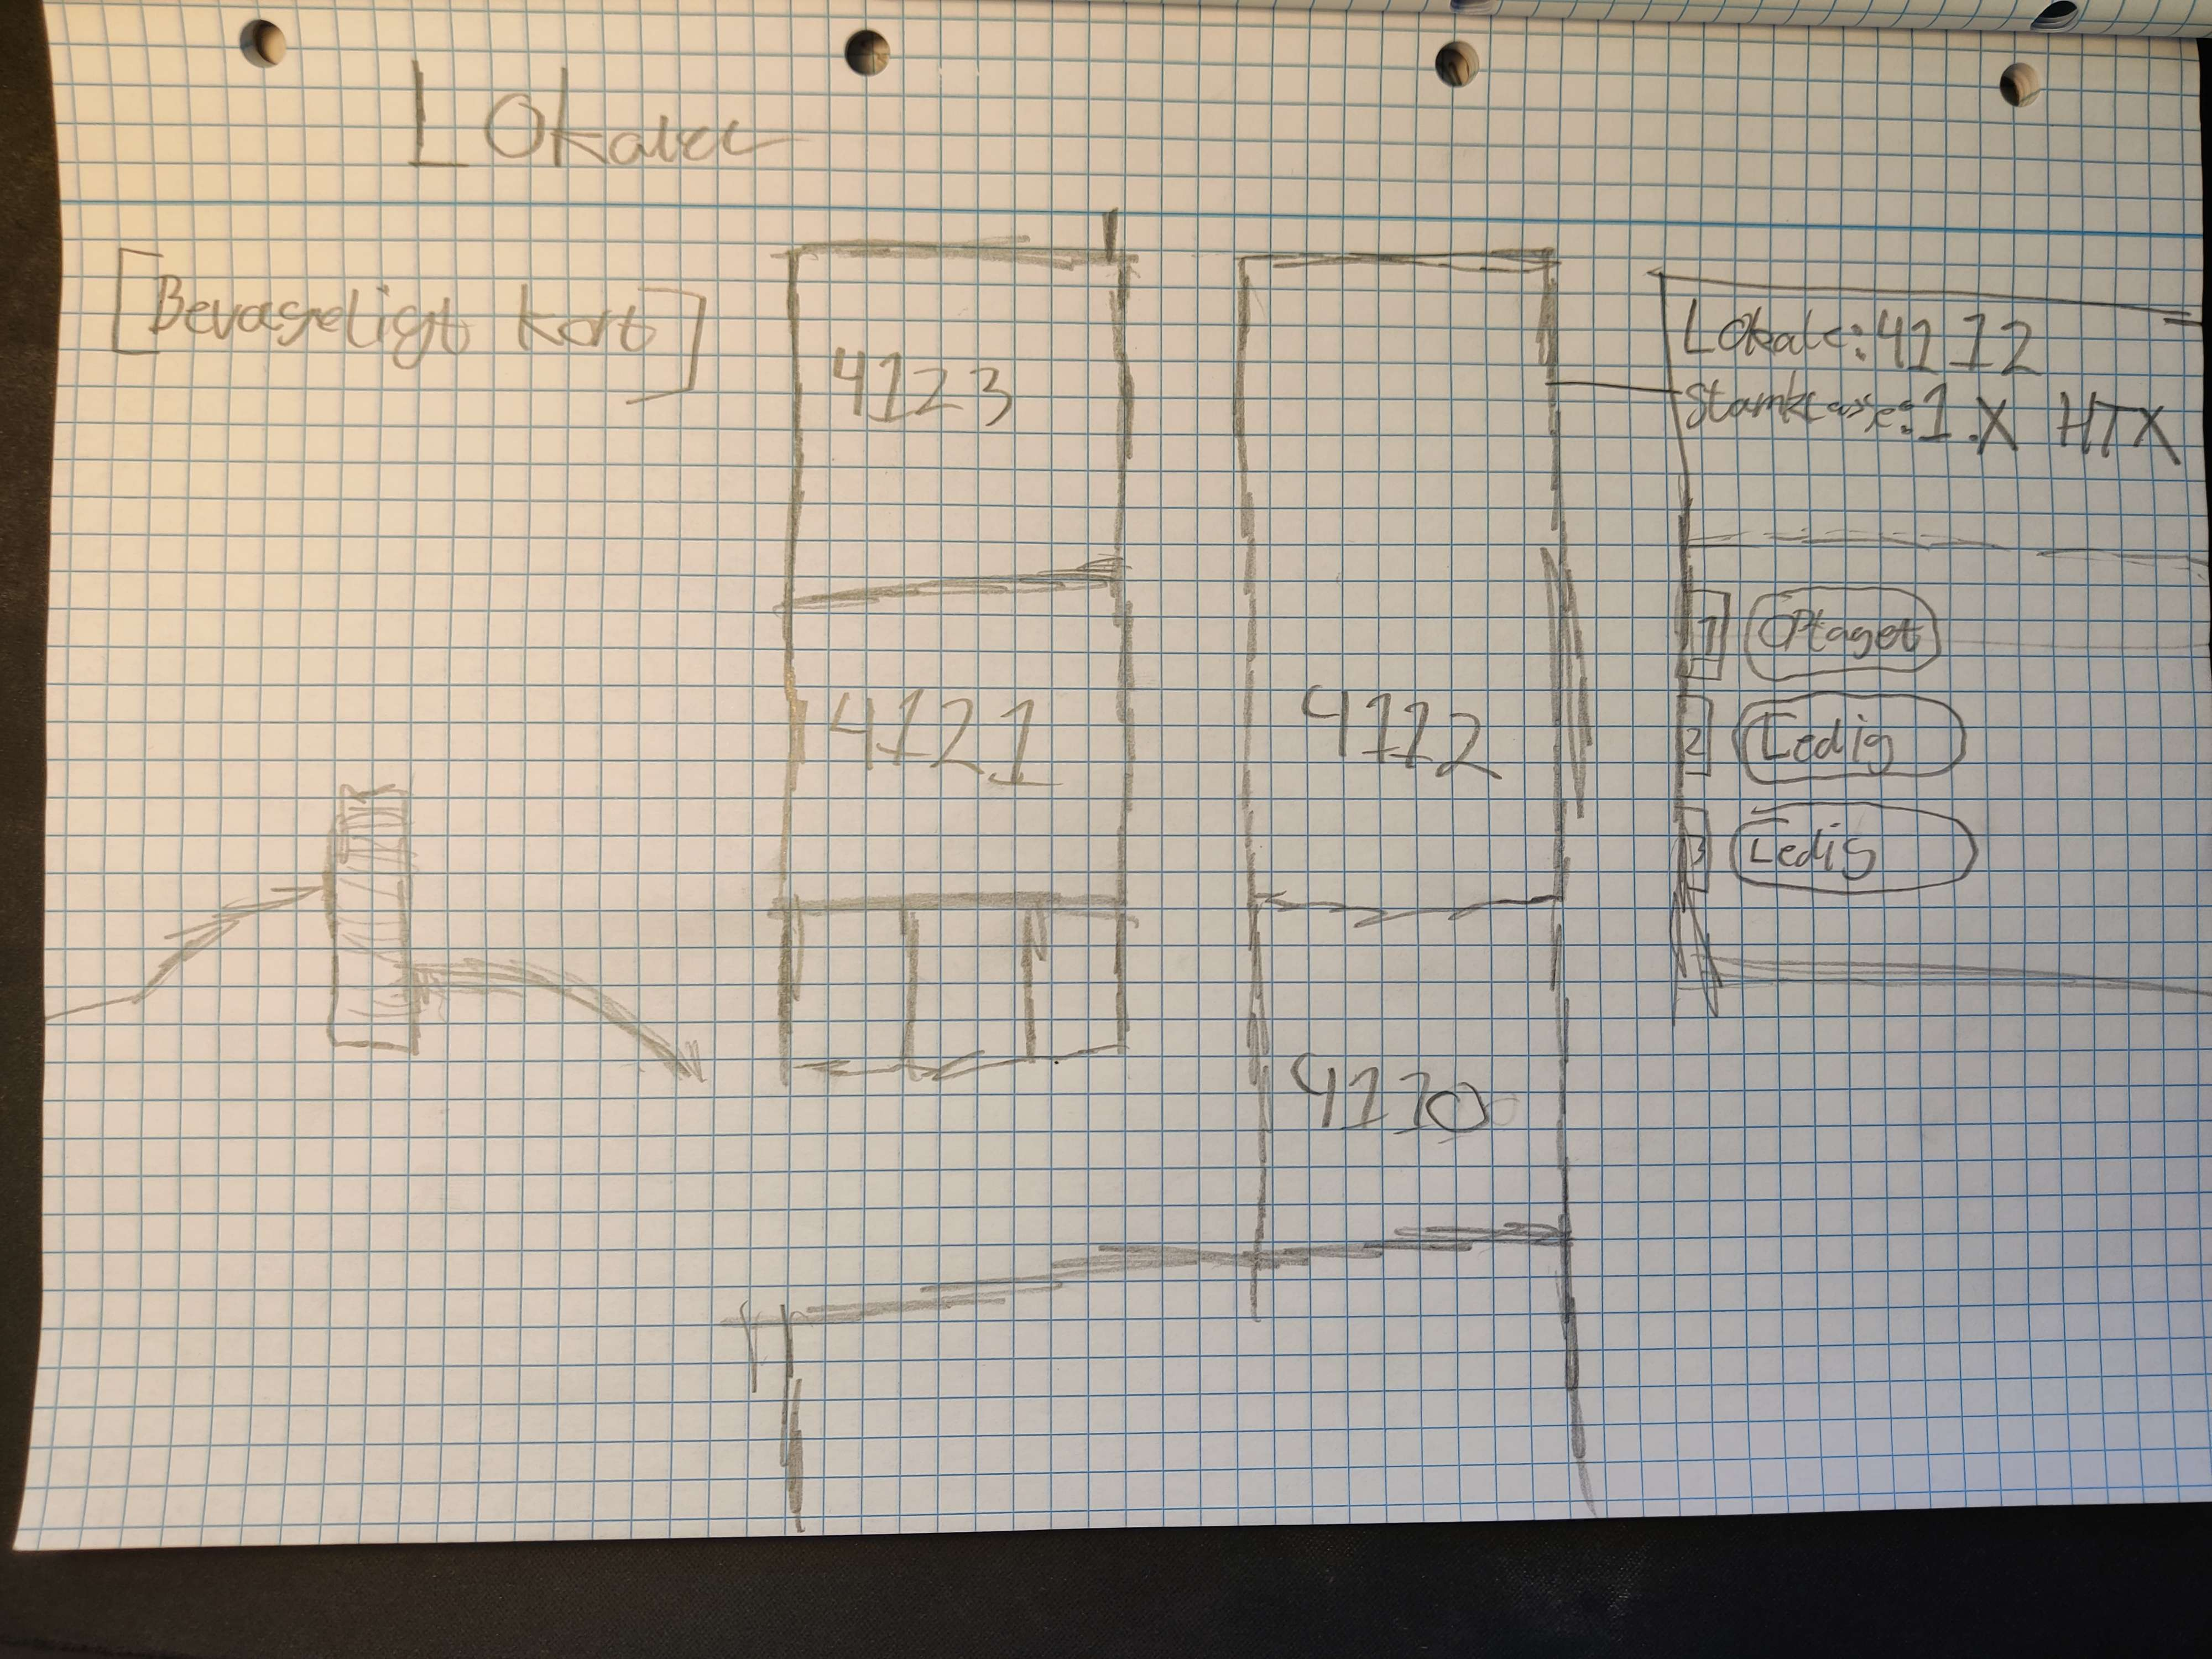
\includegraphics{assets/lectio_lokaler_skitse.jpg}}
            \caption{Viser Skitse af Booking siden på samme webapplikation som Lectio Reworket}
        \end{figure}
         \newpage
    \newpage
%% Back matter
    \printbibliography[heading=bibintoc,title={Litteraturliste}]
    \begin{appendices} \newpage
        \section{Projektbeskrivelse \label{appendix:projektbeskrivelse}} \newpage
        \renewcommand*{\thepage}{A\arabic{page}}
        
\includepdf[pages=-,delta=5 5,frame=true,landscape=true,nup=1x2,pagecommand={\thispagestyle{plain}}]{appendix/Project description/project-description.pdf}
        \renewcommand*{\thepage}{\arabic{page}}
        \section{Logbog} \newpage
        \renewcommand*{\thepage}{B\arabic{page}}
        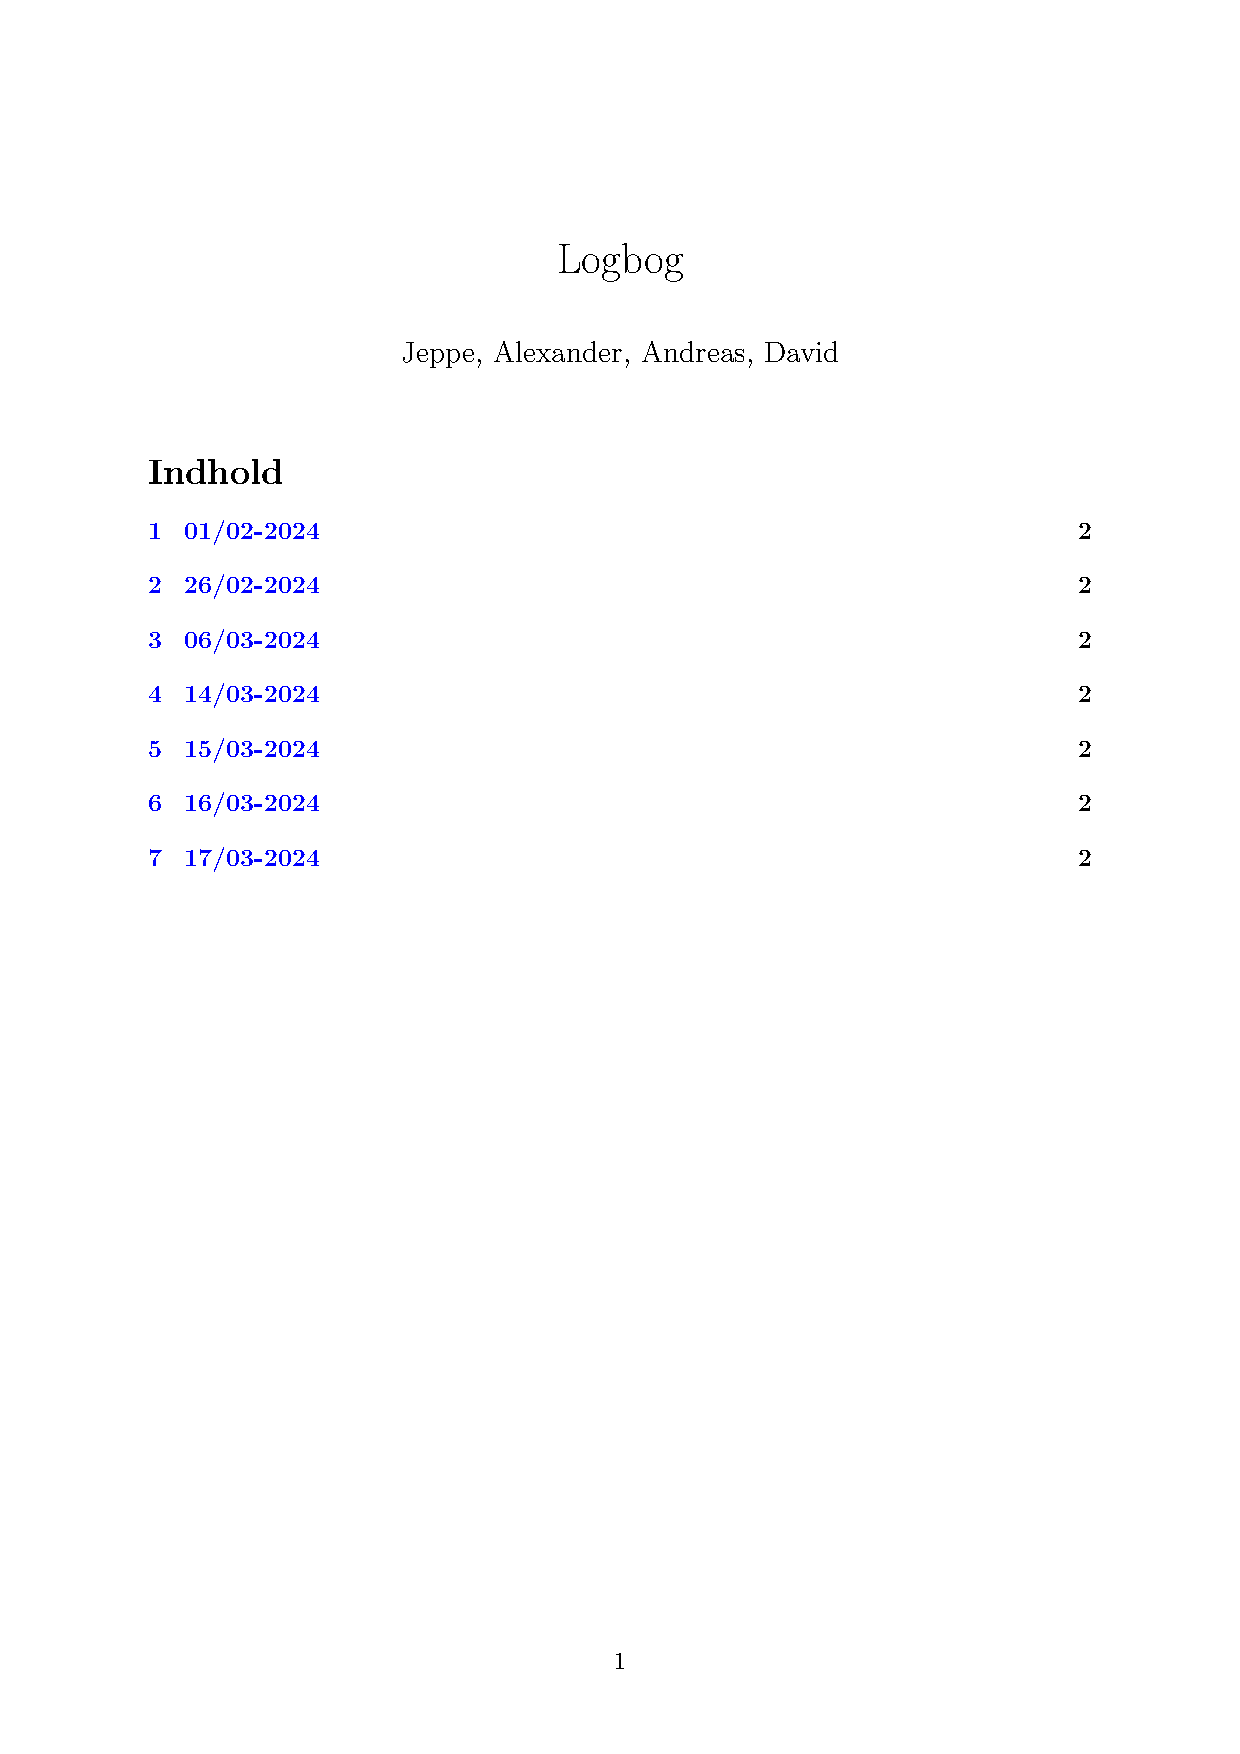
\includepdf[pages=-,delta=5 5,frame=true,landscape=true,nup=1x2,pagecommand={\thispagestyle{plain}}]{Log/log.pdf}
        \renewcommand*{\thepage}{\arabic{page}}
    \end{appendices}
\end{document}
